\documentclass{beamer}
\usepackage[utf8]{inputenc}
%\usepackage[T1]{fontenc}
\usepackage{subcaption}
\usepackage{wrapfig}
\usepackage[english,polish]{babel}

\graphicspath{ {images/} {images/collisions24x10_2x2} }

\usetheme{CambridgeUS}

\title{Modelowanie elastycznych i nieelastycznych zderzeń obiektów 
metodą dynamiki molekularnej na potrzeby animacji komputerowych}
    \subtitle{Prezentacja wybranych elementów}
    \author[Kamil Pasterczyk]{Kamil Pasterczyk \and \\ Promotor: dr hab. inż. Tomasz Chwiej}
    \institute[AGH]{AGH University of Science and Technology}
\date{\today}


\begin{document}

\section{Praca magisterska}
\subsection{Prezentacja wybranych elementów}

\begin{frame}
    \titlepage
\end{frame}

\begin{frame}
    \frametitle{Połączenia międzywęzłowe}

    \begin{figure}[h]
        \begin{subfigure}{0.45\textwidth}
            \centering
            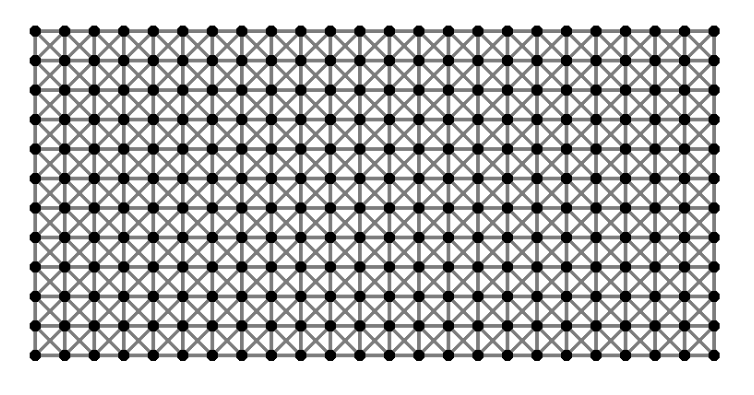
\includegraphics[width=5.5cm]{12x24}
        \end{subfigure}
        \begin{subfigure}{0.45\textwidth}
            \centering
            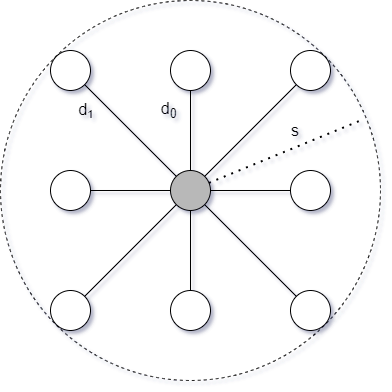
\includegraphics[width=4.5cm]{connections.drawio}
        \end{subfigure}
    \end{figure}

    Dla każdego węzła znajdujemy wszystkie węzły w odległości $s$, i dodajemy do listy połączeń wraz z informacją
    w jakiej odległości od siebie się znajdują ($d_0$, $d_1$). W ten sposób możemy stworzyć elastyczny obiekt, kształt
    zostanie zachowany.
\end{frame}

\begin{frame}
    \frametitle{Model}
    Potencjał Lennarda-Jonesa został wykorzystany do symulacji przyciągania/odpychania węzłów w jednym obiekcie,
    symulacji kolizji węzłów ze ścianami oraz symulacji kolizji węzłów z węzłami należącymi
    do innych obiektów. Wzór na siłę pomiędzy dwoma węzłami wynikającą z potencjału Lennarda-Jonesa wygląda następująco:
    \begin{equation}
        F_{LJ} = 3\frac{V_0}{d_0} \left[ \left(\frac{d_0}{l}\right)^{7} - \left(\frac{d_0}{l}\right)^{13} \right]
    \end{equation}

    Gdzie $l$ to odległość między dwiema oddziałującymi cząstkami, $V_0$ to współczynnik określający wartość potencjału.
    Potencjał Lennarda-Jonesa ma swoje minimum w odległości $d_0$, na tej odległości siła wypadkowa jest zerowa.
\end{frame}

\begin{frame}
    \frametitle{Widok aplikacji}
    \begin{figure}[H]
        \centering
        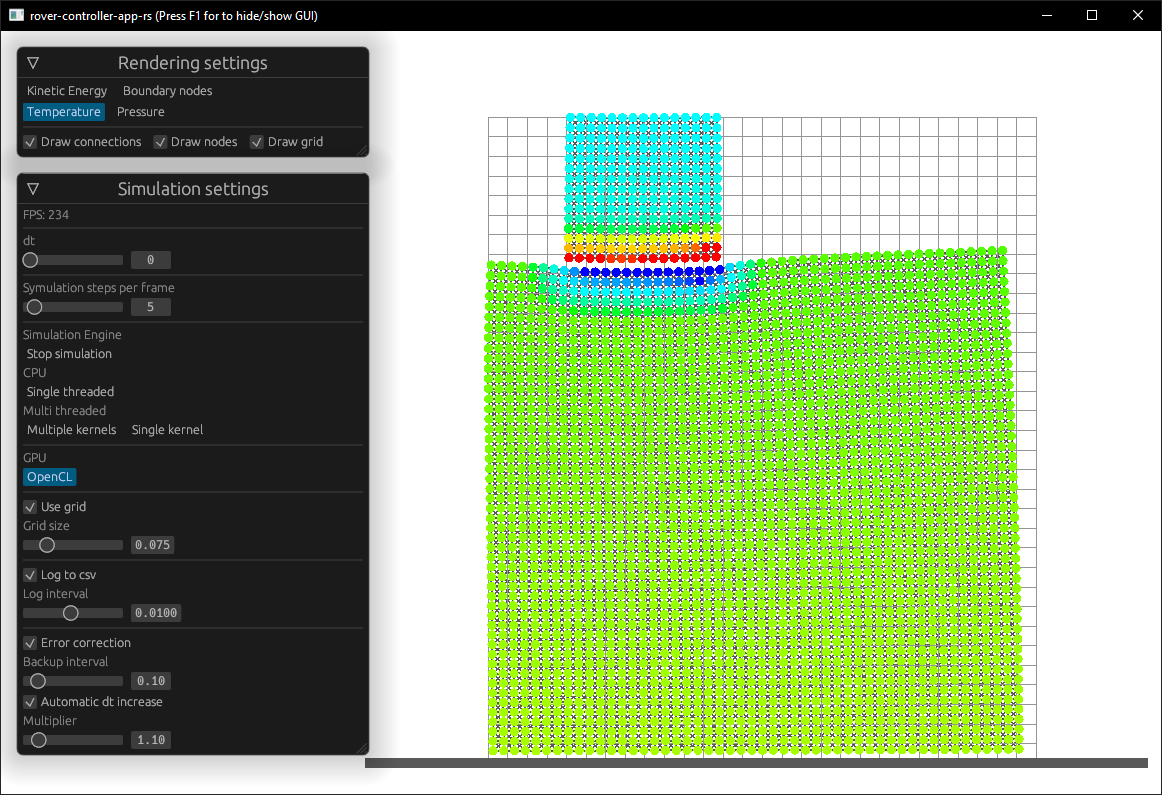
\includegraphics[width=9.5cm]{app_view_full.png}
        \caption{Okno aplikacji z widocznymi panelami ustawień}
    \end{figure}
\end{frame}


\begin{frame}
    \frametitle{Przykład zderzenia - rozerwanie obiektów}
    \begin{figure}[h]

        \begin{subfigure}{0.4\textwidth}
            \centering
            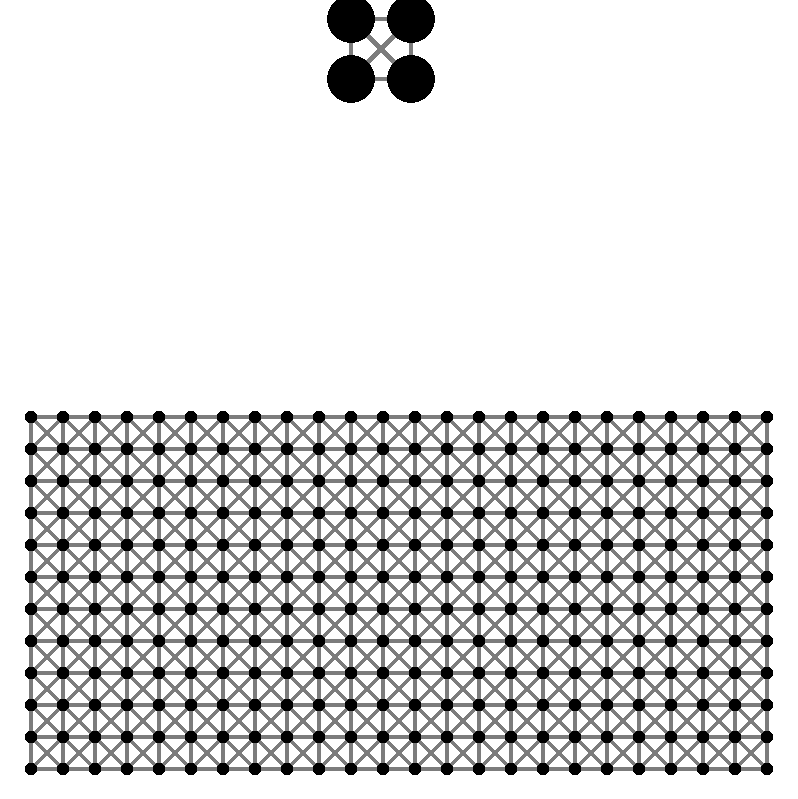
\includegraphics[width=1.7cm, height=1.7cm]{collision_2x2_24x12_mass80_1}
            \caption{Stan początkowy}
        \end{subfigure}
        \begin{subfigure}{0.4\textwidth}
            \centering
            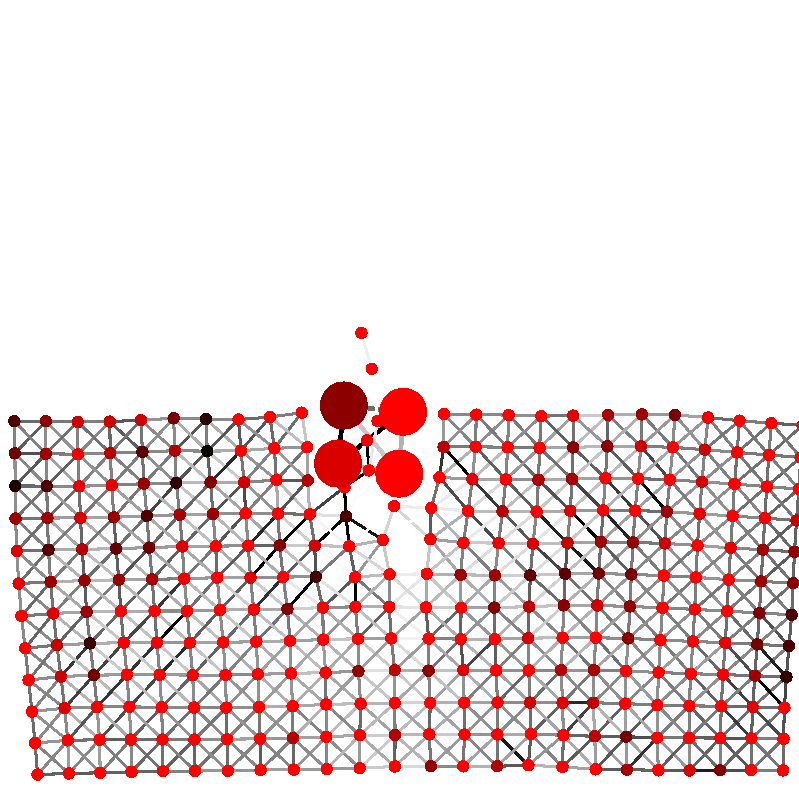
\includegraphics[width=1.7cm, height=1.7cm]{collision_2x2_24x12_mass80_2}
            \caption{Zderzenie}
        \end{subfigure}
        \begin{subfigure}{0.4\textwidth}
            \centering
            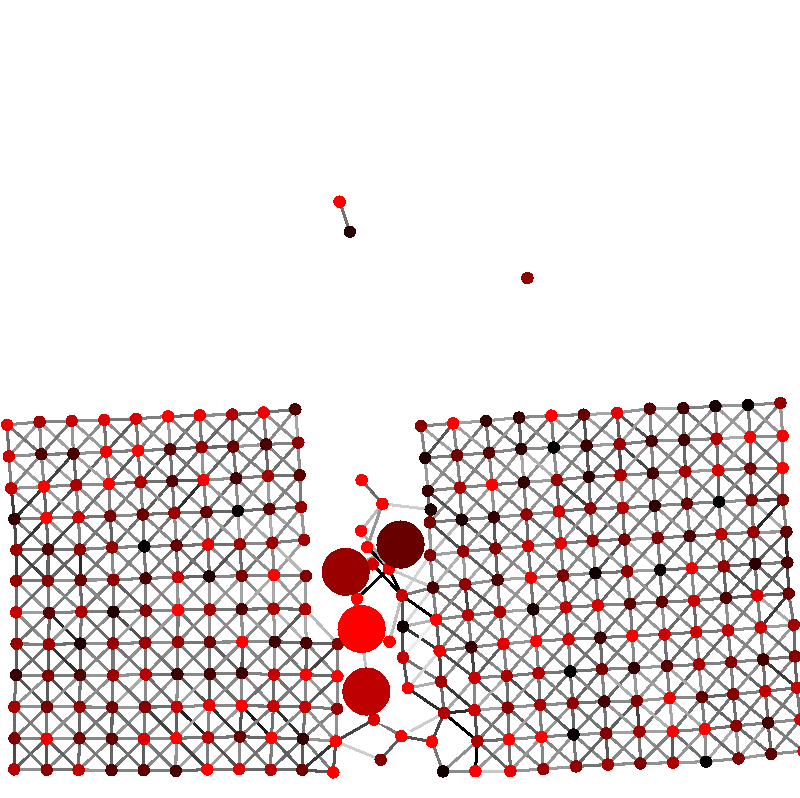
\includegraphics[width=1.7cm, height=1.7cm]{collision_2x2_24x12_mass80_3}
            \caption{Chwila po zderzeniu}
        \end{subfigure}
        \begin{subfigure}{0.4\textwidth}
            \centering
            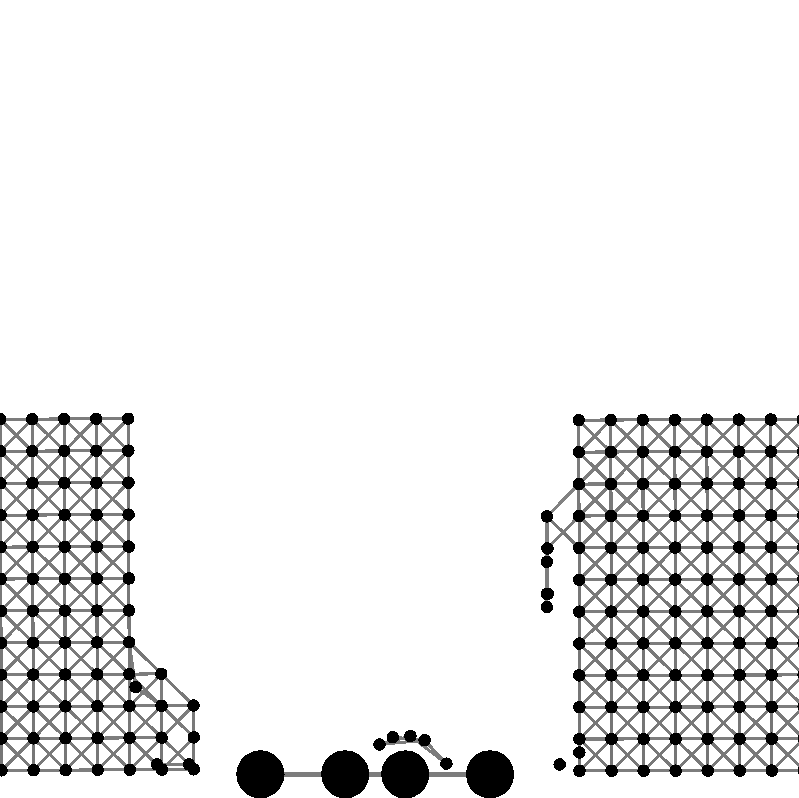
\includegraphics[width=1.7cm, height=1.7cm]{collision_2x2_24x12_mass80_4}
            \caption{Stan stabilny}
        \end{subfigure}

        \caption{Zderzenie spadającego obiektu $2 \times 2$ o masie 320 kg na obiekt $12 \times 24$ o masie 288 kg}
    \end{figure}

    Widoczna jest fala energii kinetycznej a same obiekty zostają rozerwane.
\end{frame}

\begin{frame}
    \frametitle{Przykład zderzenia - bez zniszczeń}
    \begin{figure}[h]

        \begin{subfigure}{0.4\textwidth}
            \centering
            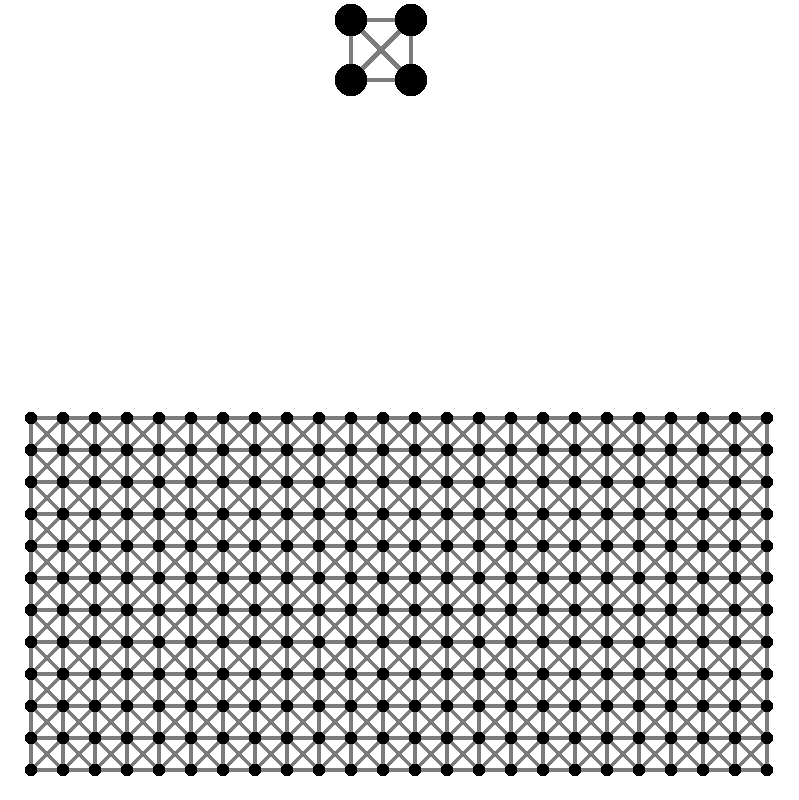
\includegraphics[width=1.7cm, height=1.7cm]{collision_2x2_24x12_mass30_1}
            \caption{Stan początkowy}
        \end{subfigure}
        \begin{subfigure}{0.4\textwidth}
            \centering
            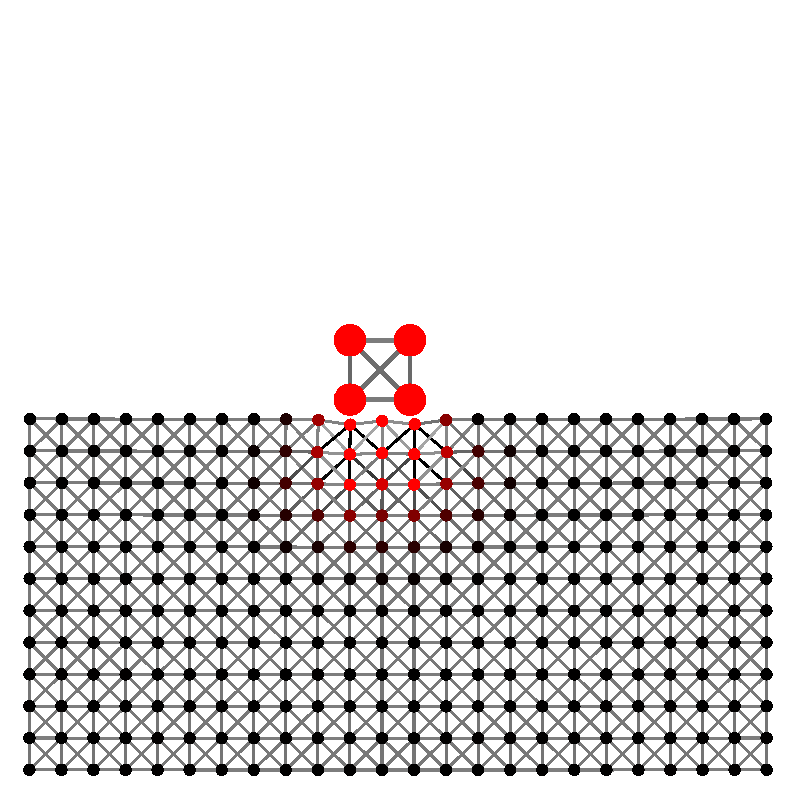
\includegraphics[width=1.7cm, height=1.7cm]{collision_2x2_24x12_mass30_2}
            \caption{Zderzenie}
        \end{subfigure}
        \begin{subfigure}{0.4\textwidth}
            \centering
            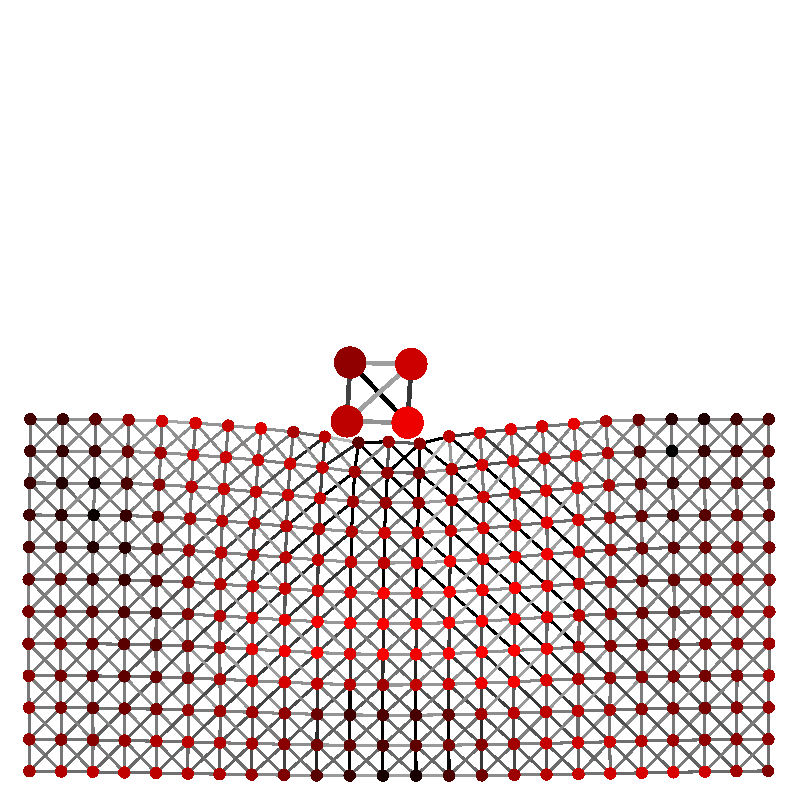
\includegraphics[width=1.7cm, height=1.7cm]{collision_2x2_24x12_mass30_3}
            \caption{Chwila po zderzeniu}
        \end{subfigure}
        \begin{subfigure}{0.4\textwidth}
            \centering
            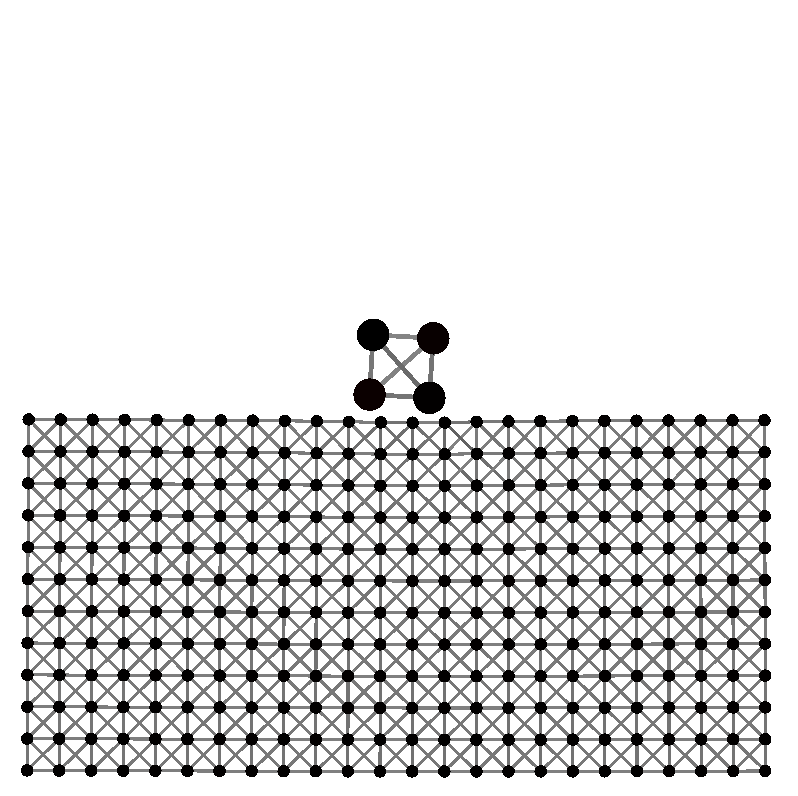
\includegraphics[width=1.7cm, height=1.7cm]{collision_2x2_24x12_mass30_4}
            \caption{Stan stabilny}
        \end{subfigure}

        \caption{Zderzenie spadającego obiektu $2 \times 2$ o masie 120 kg na obiekt $12 \times 24$ o masie 288 kg}
    \end{figure}

    Węzły zmieniają kolor z czarnego na czerwony wraz z wzrostem ich energii kinetycznej.
\end{frame}


\begin{frame}
    \frametitle{Test poprawności - zachowanie energii}

    Dwa obiekty o rozmiarach $8 \times 8$ i $6 \times 4$ znajdują się w polu grawitacyjnym, 
    nie występują siły oporu/tarcia.

    \begin{figure}[H]
        \centering
        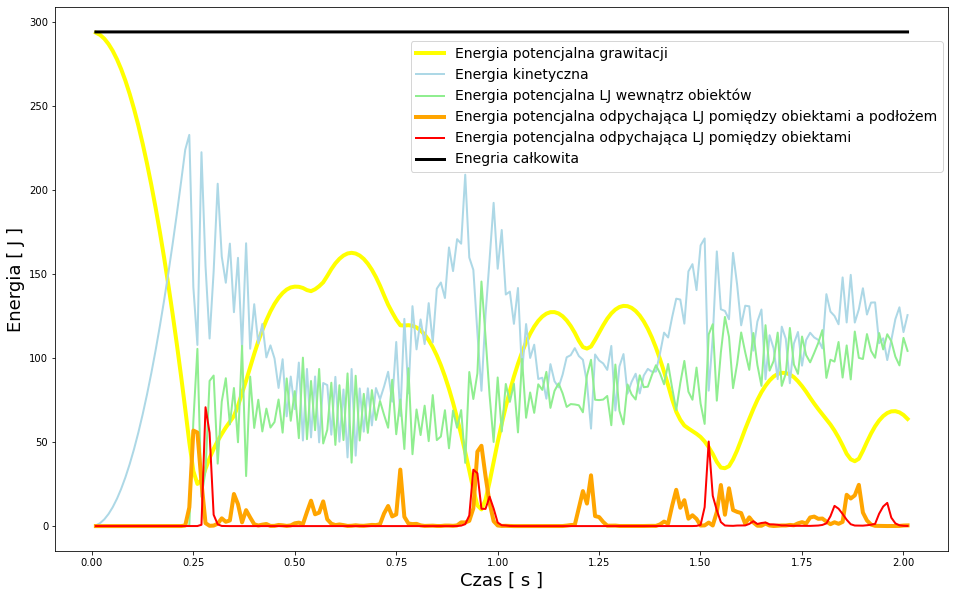
\includegraphics[width=8.8cm]{energy_test_0to2s.png}
        \caption{Zmiana energii w czasie dla układu w ciągu pierwszych 1.2 sekund}
    \end{figure}

\end{frame}


\begin{frame}
    \frametitle{Tryby kolorowania węzłów}

    \begin{figure}[h]

        \begin{subfigure}{0.4\textwidth}
            \centering
            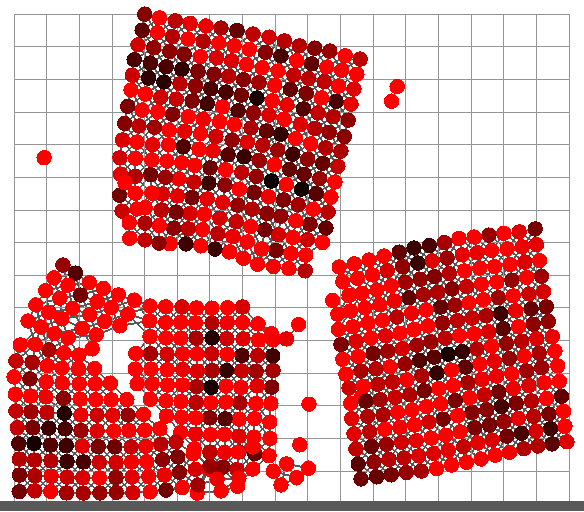
\includegraphics[width=2.5cm]{app_kinetic_view.png} 
            \caption{Energia kinetyczna}
        \end{subfigure}
        \begin{subfigure}{0.4\textwidth}
            \centering
            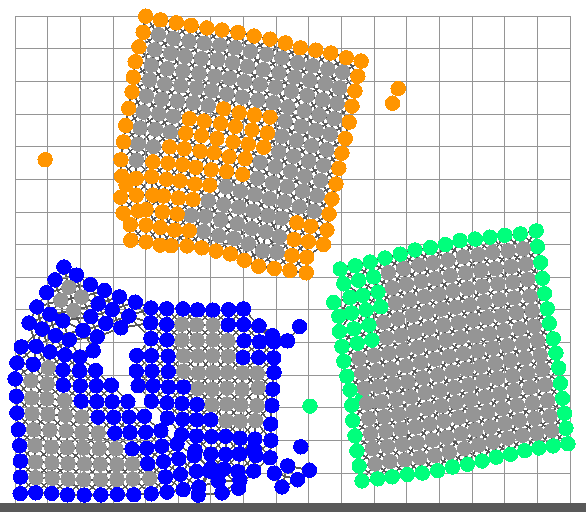
\includegraphics[width=2.5cm]{app_boundary_view.png}
            \caption{Węzły brzegowe}
        \end{subfigure}
        \begin{subfigure}{0.4\textwidth}
            \centering
            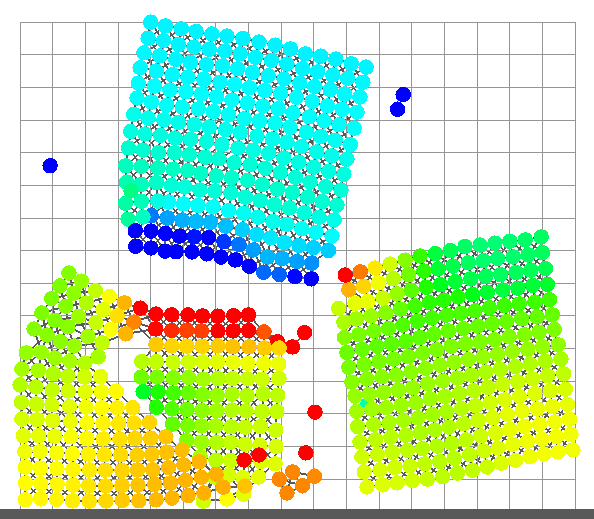
\includegraphics[width=2.5cm]{app_temperature_view.png}
            \caption{Temperatura}
        \end{subfigure}
        \begin{subfigure}{0.4\textwidth}
            \centering
            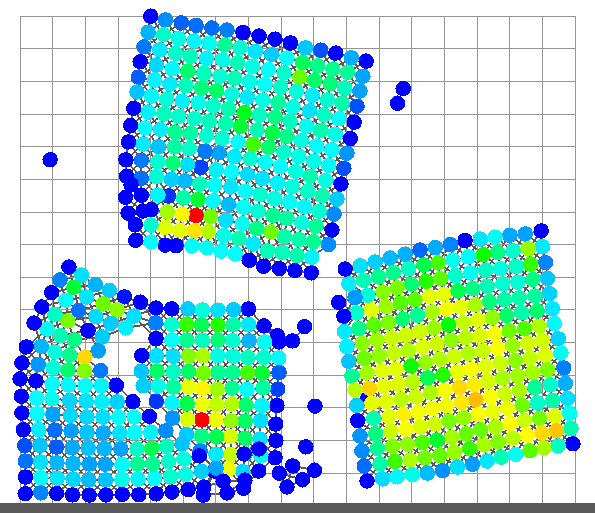
\includegraphics[width=2.5cm]{app_pressure_view.png}
            \caption{Ciśnienie}
        \end{subfigure}
        
        \caption{Porównanie widoków tej samej sceny w kilku trybach kolorowania węzłów}
    \end{figure}

\end{frame}

\begin{frame}
    \frametitle{Wizualizacja ciśnienia - przypadek statyczny}

    \begin{figure}[h]
        \begin{subfigure}{0.4\textwidth}
            \centering
            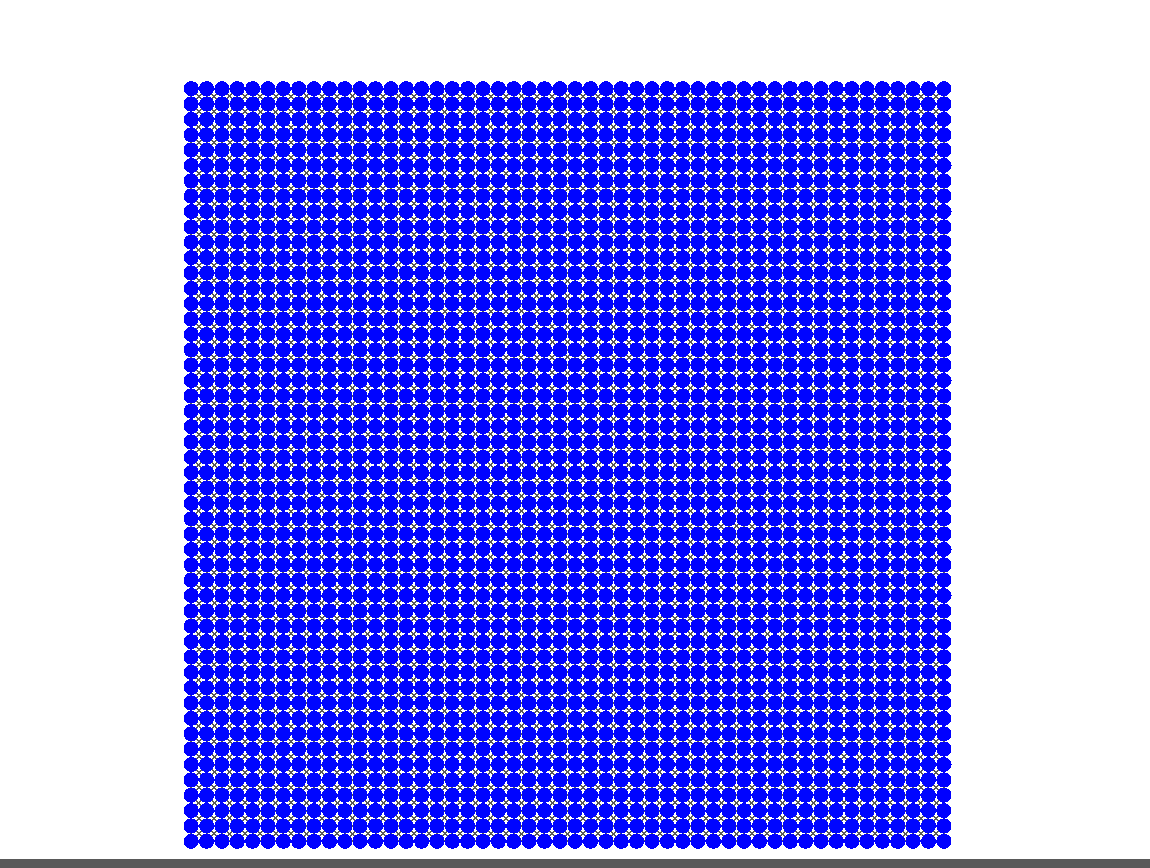
\includegraphics[width=2.5cm]{pressure_01.png} 
            \caption{Stan początkowy}
        \end{subfigure}
        \begin{subfigure}{0.4\textwidth}
            \centering
            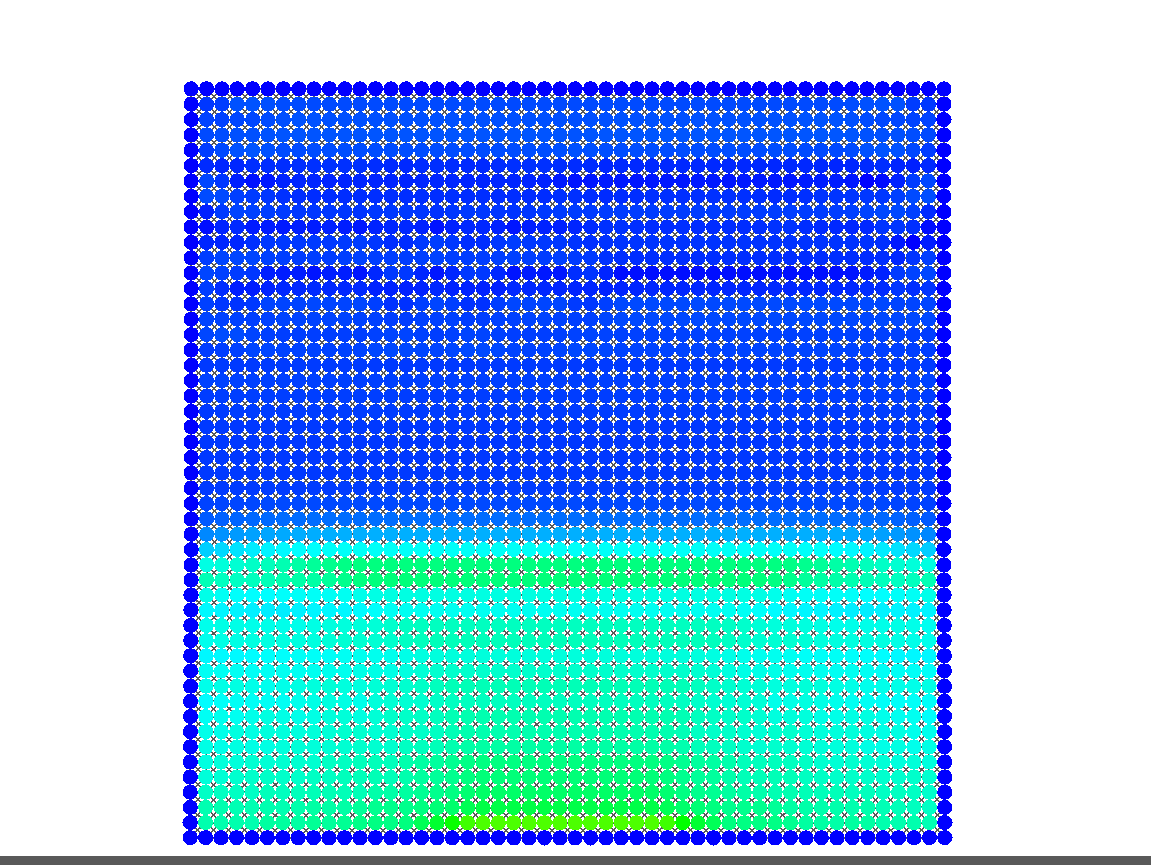
\includegraphics[width=2.5cm]{pressure_02.png}
            \caption{Przed zderzeniem}
        \end{subfigure}
        \begin{subfigure}{0.4\textwidth}
            \centering
            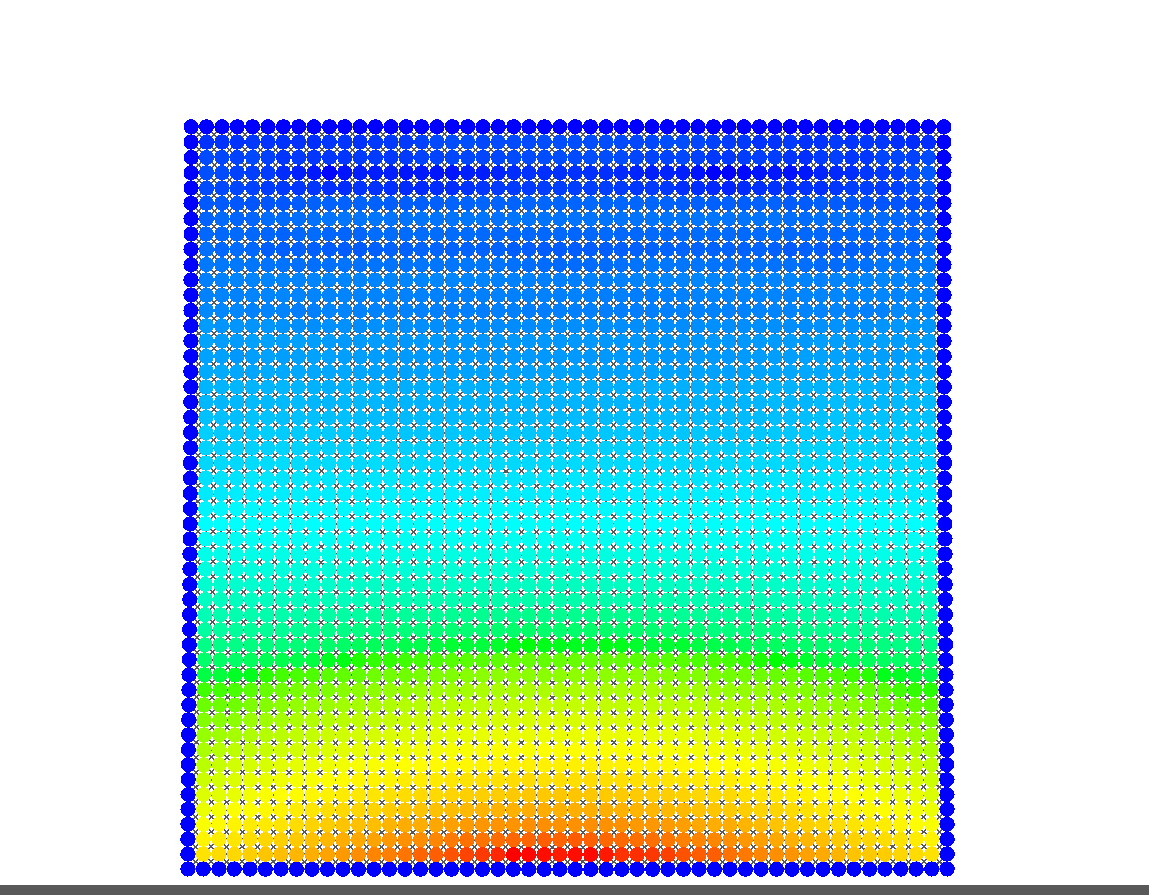
\includegraphics[width=2.5cm]{pressure_03.png}
            \caption{Zderzenie}
        \end{subfigure}
        \begin{subfigure}{0.4\textwidth}
            \centering
            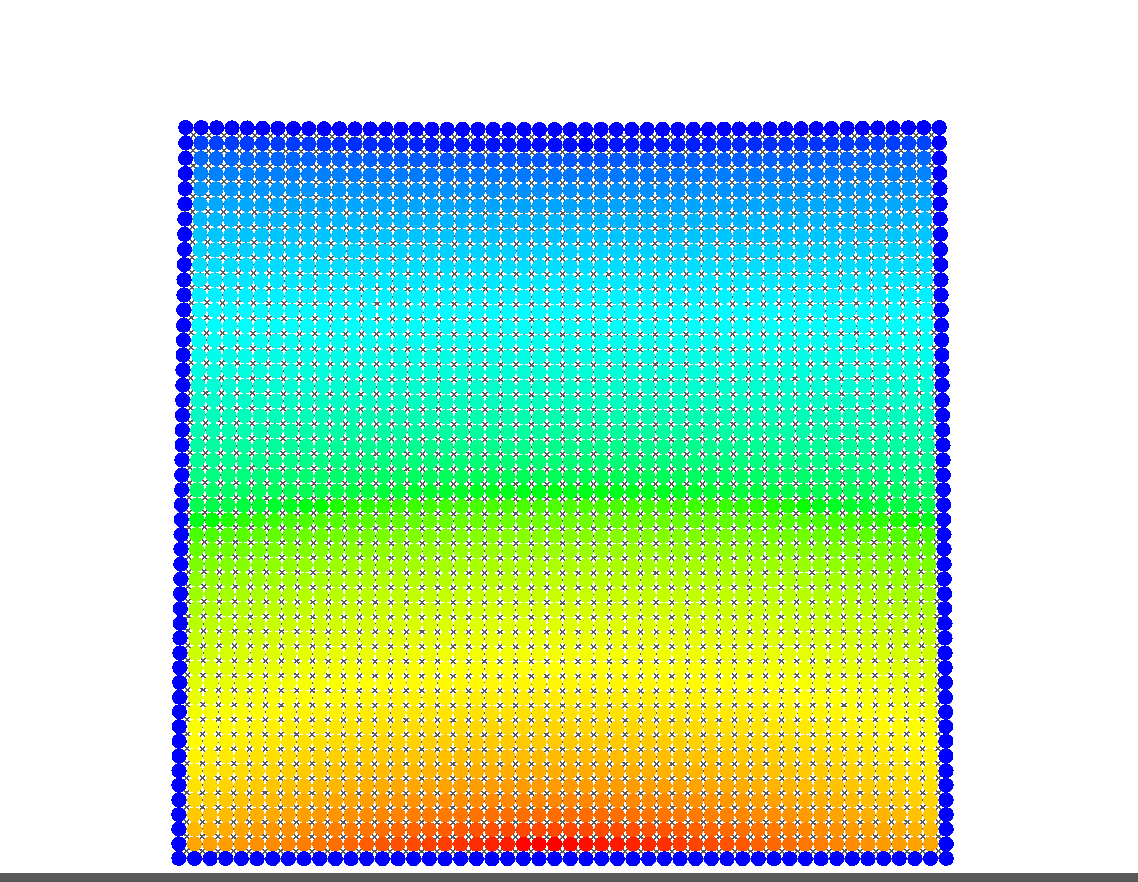
\includegraphics[width=2.5cm]{pressure_04.png}
            \caption{Stan stabilny}
        \end{subfigure}
        
        \caption{Widok ciśnienia w wybranych chwilach czasowych dla obiektu $50 \times 50$}
    \end{figure}

\end{frame}

\begin{frame}
    \frametitle{Zmiana energii układu w czasie - przypadek statyczny}

    \begin{figure}[H]
        \centering
        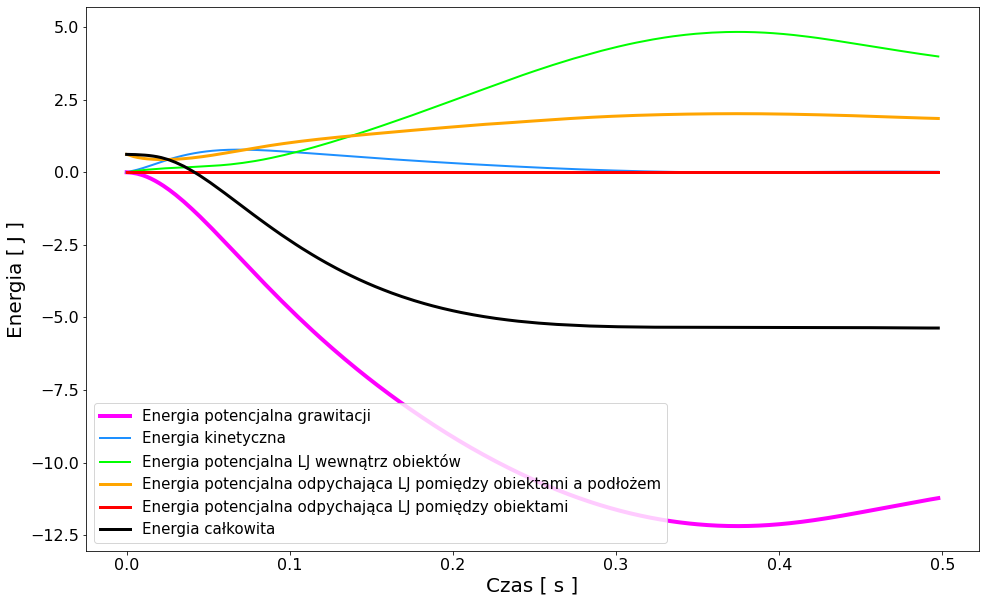
\includegraphics[width=10.5cm]{pressure_energy_01}
        \caption{
            Zmiana energi układu w czasie dla pierwszych 0.5 sekundy
        }
    \end{figure}
\end{frame}

\begin{frame}
    \frametitle{Wizualizacja ciśnienia - przypadek dynamiczny}

    \begin{figure}[h]
        \begin{subfigure}{0.4\textwidth}
            \centering
            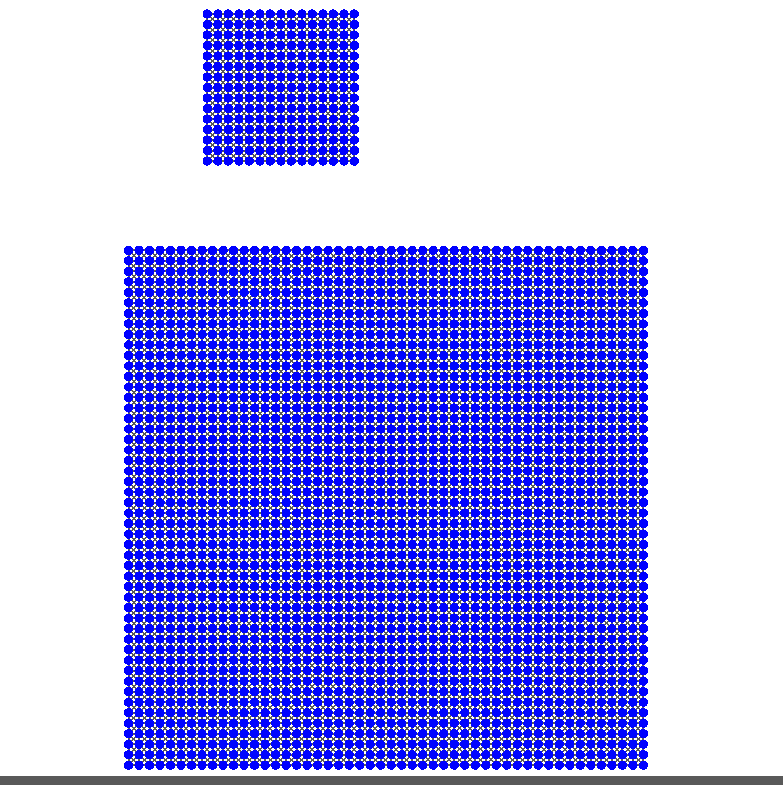
\includegraphics[width=2.3cm]{pressure02_01} 
            \caption{Stan początkowy}
        \end{subfigure}
        \begin{subfigure}{0.4\textwidth}
            \centering
            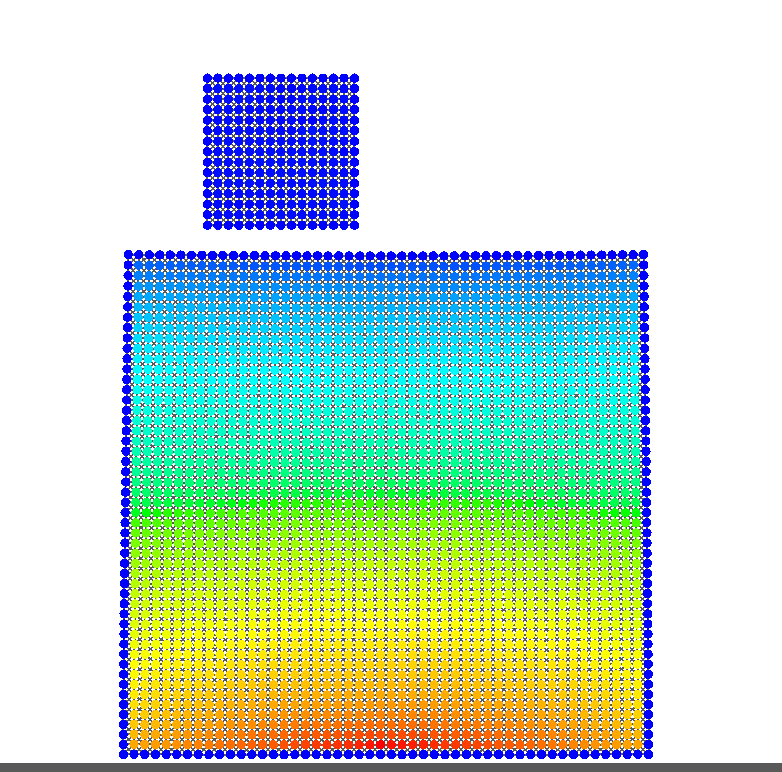
\includegraphics[width=2.3cm]{pressure02_02}
            \caption{Przed zderzeniem}
        \end{subfigure}
        \begin{subfigure}{0.4\textwidth}
            \centering
            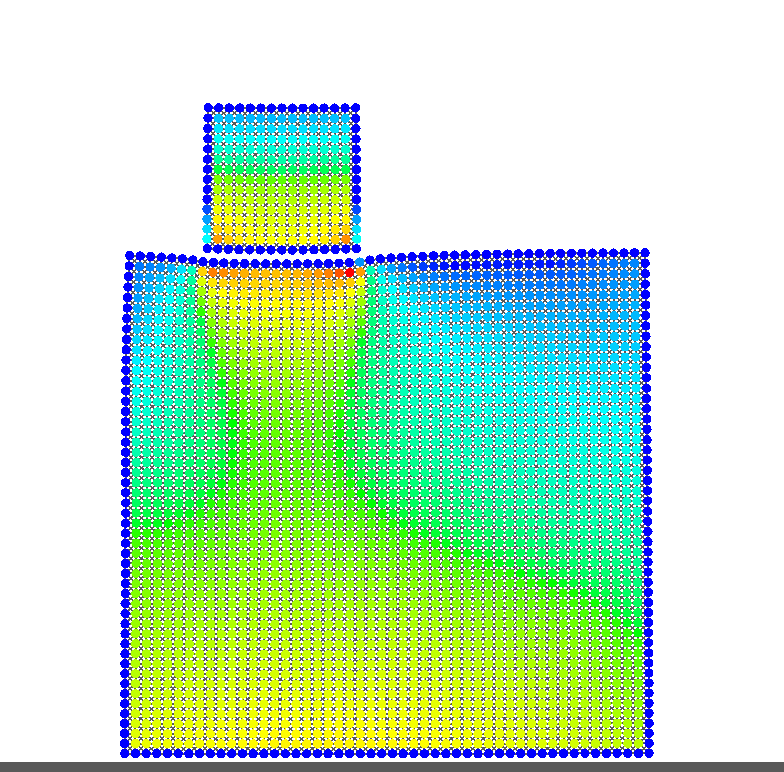
\includegraphics[width=2.3cm]{pressure02_03}
            \caption{Zderzenie}
        \end{subfigure}
        \begin{subfigure}{0.4\textwidth}
            \centering
            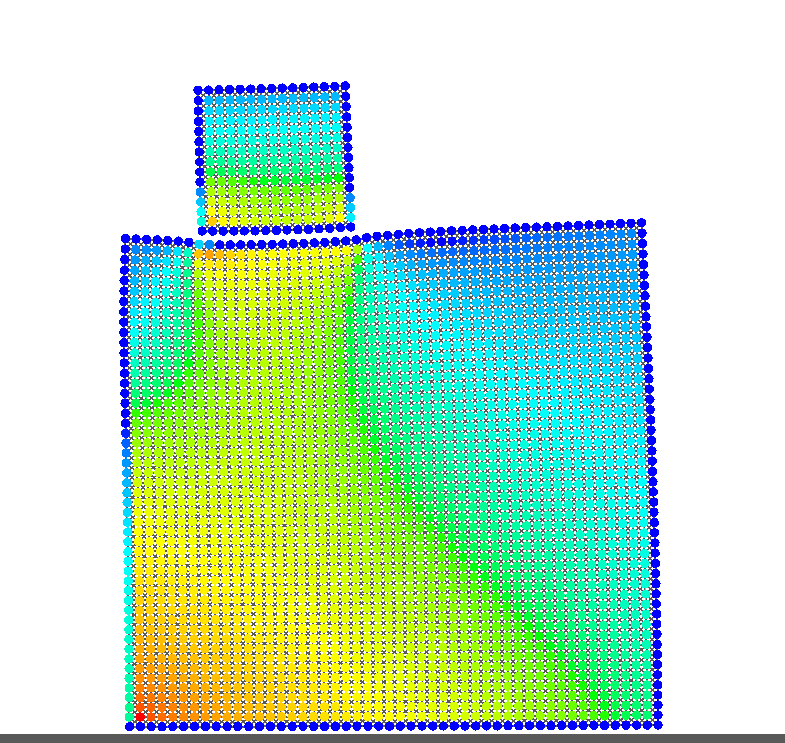
\includegraphics[width=2.3cm]{pressure02_04}
            \caption{Stan stabilny}
        \end{subfigure}
        
        \caption{Widok ciśnienia w wybranych chwilach czasowych dla zderzenia obiektów $50 \times 50$ i $20 \times 20$}
    \end{figure}

\end{frame}

\begin{frame}
    \frametitle{Zmiana energii układu w czasie - przypadek dynamiczny}

    \begin{figure}[H]
        \centering
        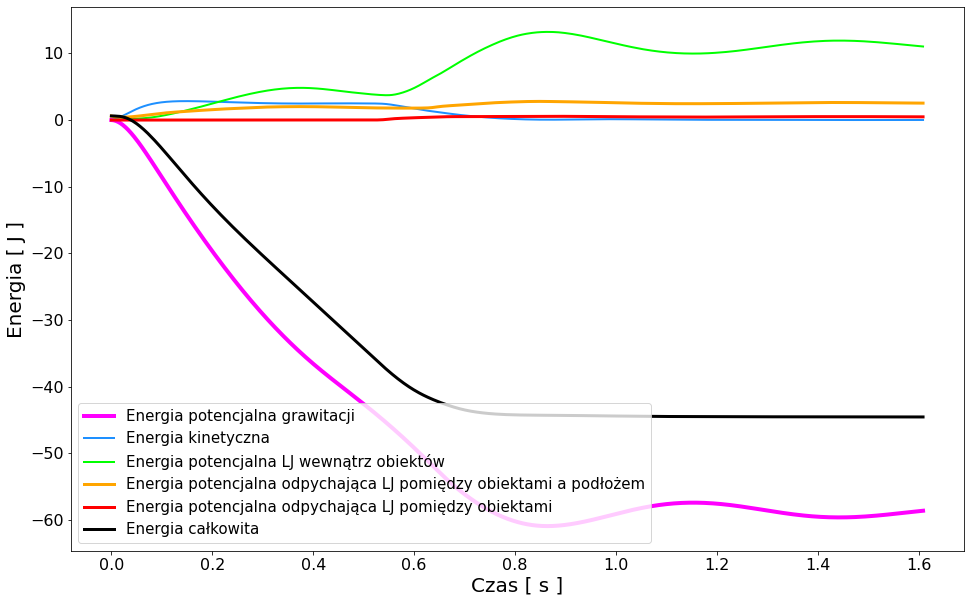
\includegraphics[width=10.5cm]{pressure_energy02_02}
        \caption{
            Zmiana energi układu w czasie dla pierwszych 1.6 sekundy
        }
    \end{figure}
\end{frame}


\begin{frame}
    \frametitle{Testy wydajności algorytmów z rozrywaniem obiektów}
    \begin{wrapfigure}{r}{0.3\textwidth}
        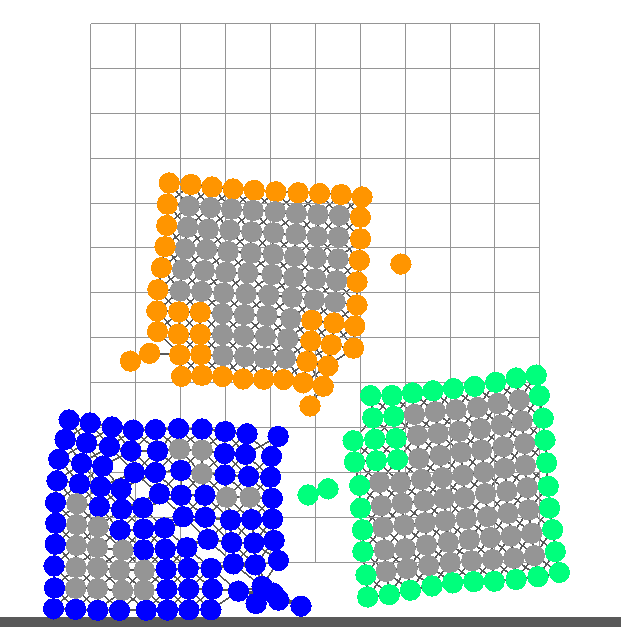
\includegraphics[width=0.9\linewidth]{app_boundary_performance_10x10_02.png} 
        \caption{Zderzenie i rozerwanie trzech obiektów $10\times10$}
    \end{wrapfigure}
    \subsection{Opis testu}
    Scena składa się z trzech obiektów zawieszonych nad podłożem na różnych wysokościach. Siła grawitacji 
    powoduje swobodny spadek tych obiektów a następnie zderzanie się i ich rozrywanie. Liczba węzłów jest
    stopniowo zwiększana poprzez zwiększanie gęstości każdego z trzech obiektów. Ilość węzłów w boku każdego 
    z tych obiektów wynosi kolejno 5, 10, 15, 25, 40, 50, 60, 75, 90, 100. \\
    
    Krok czasowy symulacji wynosi
    $2 \times 10^{-5}$ sekundy a czas trwania symulacji to $0.5$ sekundy, co 
    daje $25000$ kroków symulacji dla każdego przypadku. \\
\end{frame}



\begin{frame}
    \frametitle{Porównanie wydajności CPU}

    \begin{figure}[H]
        \centering
        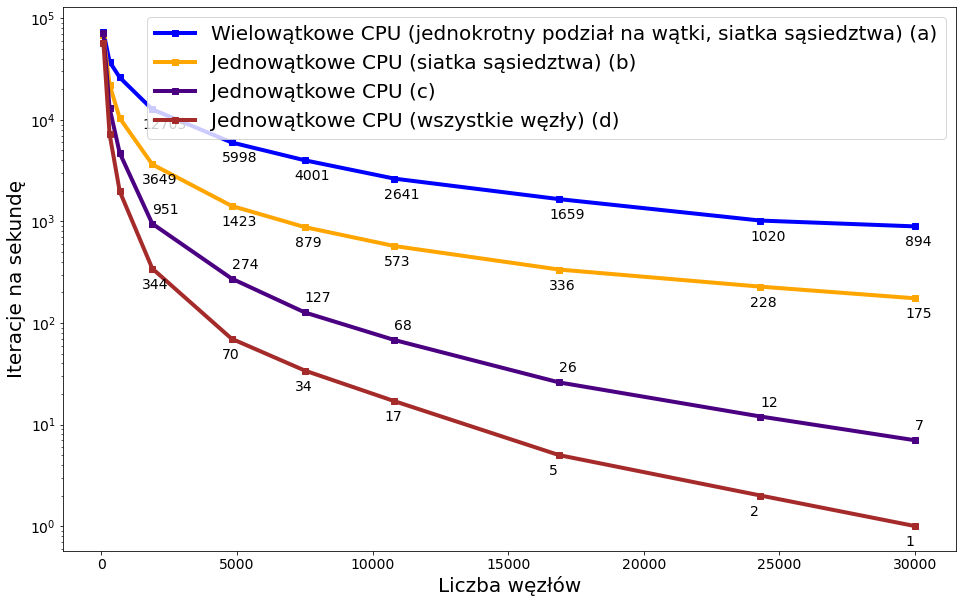
\includegraphics[width=10.5cm]{performance_all_best_worst.png}
        \caption{
            Liczba iteracji na sekundę w zależności od ilości węzłów
        }
    \end{figure}
\end{frame}

\begin{frame}
    \frametitle{Porównanie wydajności CPU i GPU}

    \begin{figure}[H]
        \centering
        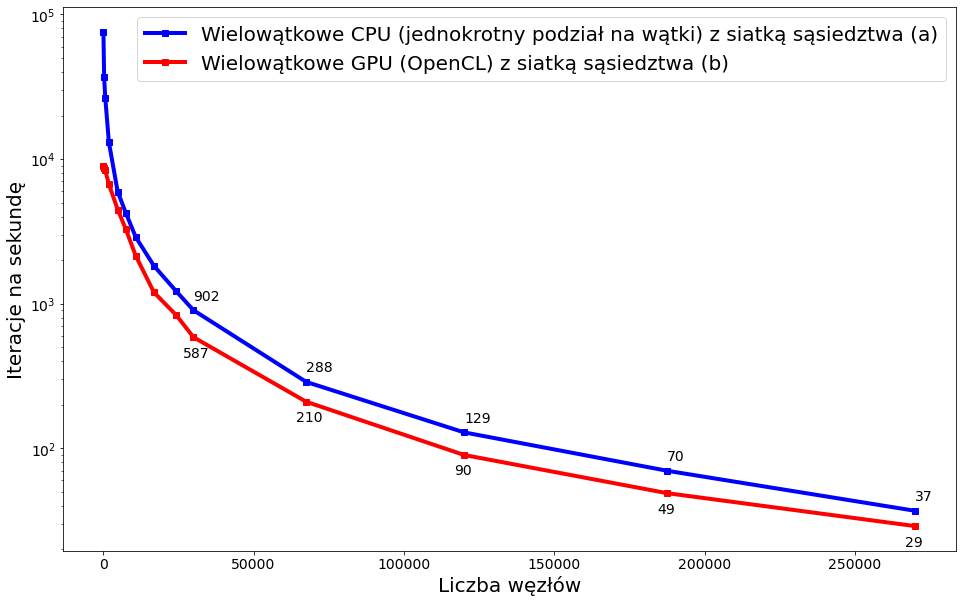
\includegraphics[width=10.5cm]{performance_best_cpu_gpu.png}
        \caption{
            Liczba iteracji na sekundę w zależności od ilości węzłów
        }
    \end{figure}
\end{frame}

\begin{frame}
    \frametitle{Koniec prezentacji}

    \centering
    \LARGE Dziękuję za uwagę!
\end{frame}

\end{document}